\documentclass[11pt]{article}
\usepackage{amsmath}
\usepackage{amssymb}
\usepackage{tikz}
\usetikzlibrary{decorations.pathreplacing}
\usetikzlibrary{math}
\usepackage{colortbl}

\begin{document}

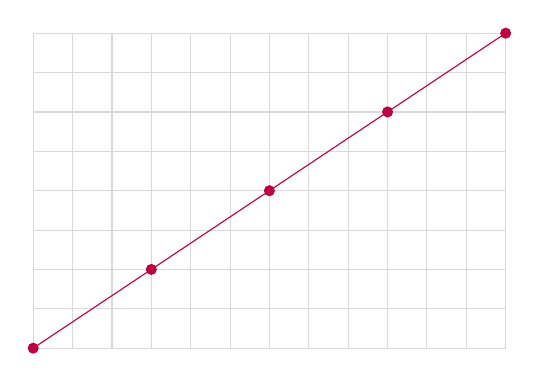
\begin{tikzpicture}[scale=0.5]
% G = 4 
    \begin{scope}[shift = {(-2,-12)}]
    % G = 4 
        \tikzmath{
        int \a, \b, \g;
        \a = 3;
        \b = 2;
        \g = 4;
        } % end tikzmath
    % grid :
        \draw[gray!30] 
            (0,0) grid (\g*\a, \g*\b);
    % boundary line:
        \draw[purple] 
            (0,0) -- (\g*\a, \g*\b); 
    % boundary points:
        \foreach \j in {0,...,\g}{
            \fill[purple]
                (\j*\a, \j*\b) circle (4pt);
        }% end foreach
    \end{scope}
\end{tikzpicture}

\end{document}